%In this work, we tuned six representative Polybench kernels for energy on
%an Intel SandyBridge processor and an Intel Xeon Phi coprocessor by applying various loop 
%transformations. For the \texttt{2mm} and \texttt{gemm} kernels (dense matrix kernels),
%we observed \emph{non-correlated} speedups and energy savings over the baseline version,
%i.e. \emph{fastest execution does not guarantee fewest energy consumption}. 
%We also showed that good loop transformations for one architecture do not carry over to
%other architectures.

%Is the above assumption true? How does a machine learning function make sure that it does 
%not give up on vectorization until everything is visible? 
%Are there relationships between optimizations that can be applied across applications?
%Can this be generalized, i.e. more apps and more optimizations?

\textbf{Evaluate the effect of putting a power cap on the system.}    


\subsection{Negative/Not Exciting Results}
Approach: we developed a unbalanced OpenMP program. The workload of a thread 
is a linear function of its thread id. 
Using gcc (v4.8.1).
We manually set the duty cycle (slowing down the threads that have fewer amount
of workload and let the thread run at full speed if the workload for it is high). 
Then we set the power cap on the system. 
Figure~\ref{fig:Unblanced} and Figure~\ref{fig:UnbalancedTime} show the results.

\begin{figure}[bt]
    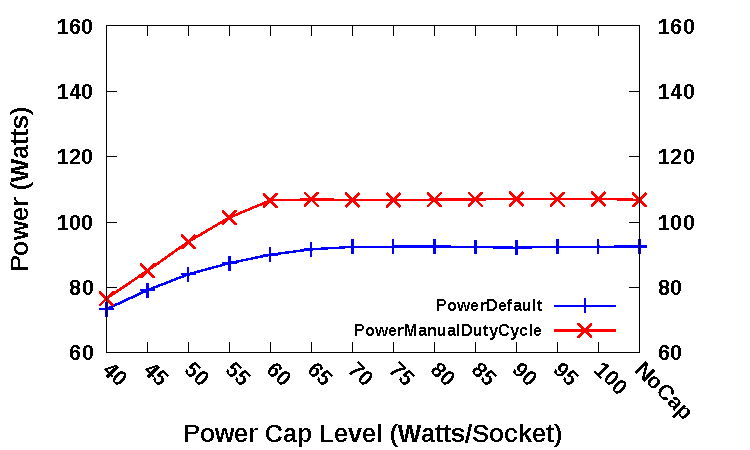
\includegraphics[width=3.5in]{orig-dutycyle-compare-power.pdf}
%    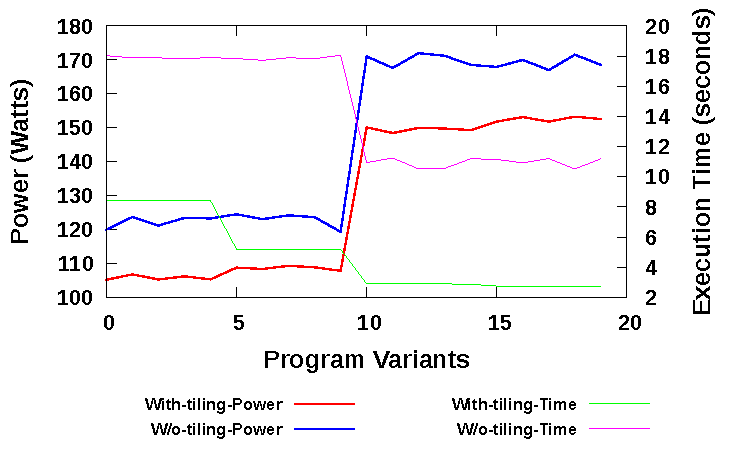
\includegraphics{Covariance}
    \caption{Power }
    \label{fig:Unbalanced}
\end{figure}
\begin{figure}[bt]
    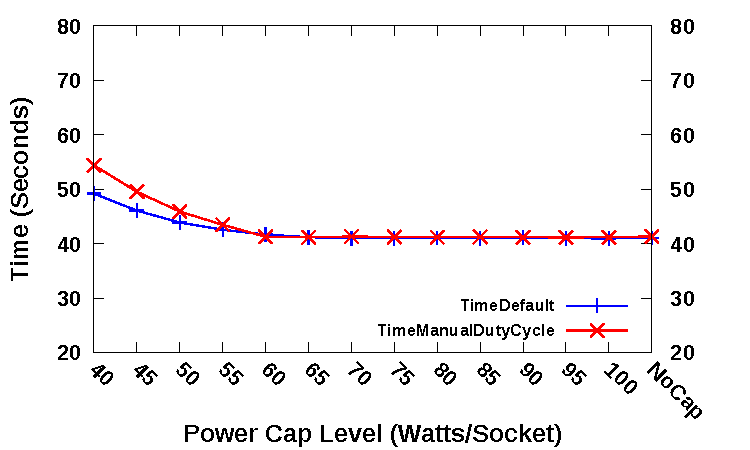
\includegraphics[width=3.5in]{orig-dutycyle-compare-time.pdf}
%    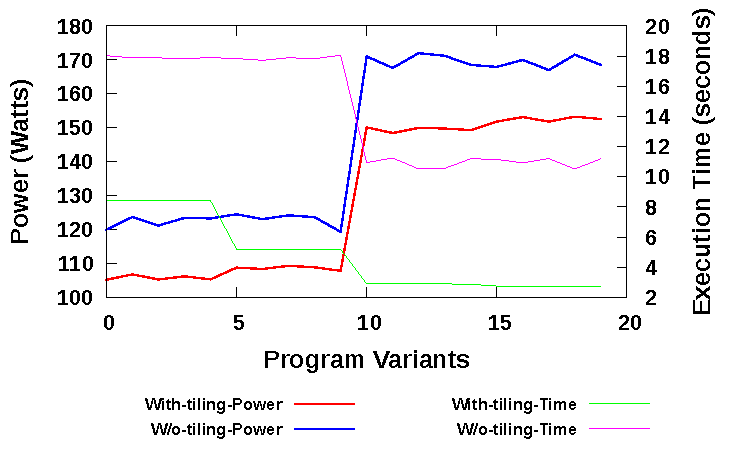
\includegraphics{Covariance}
    \caption{Time}
    \label{fig:UnbalancedTime}
\end{figure}

It shows that OpenMP program did not get benefits from slowing down some of the 
treads .

When using icc, in the case of No Cap, the results are similar:
manual duty cycle:
Application(EnergyStat) - Time 22.847241 Total energy consumed 2298.958635 Ave. Power Level 100.623032 Final Temperature socket 1 : 46  socket 2 : 37
original (wo duty cycle)
Application(EnergyStat) - Time 23.059587 Total energy consumed 2125.018620 Ave. Power Level 92.153369 Final Temperature socket 1 : 46  socket 2 : 39
Again, here the power level increase!

When I comment out the \texttt{do\_wait} function in GOMP (which is equivalent to increase GOMP\_SPIN\_COUNT-- default 3ms, very short)
The graph looks like  the following: 


\begin{figure}[bt]
    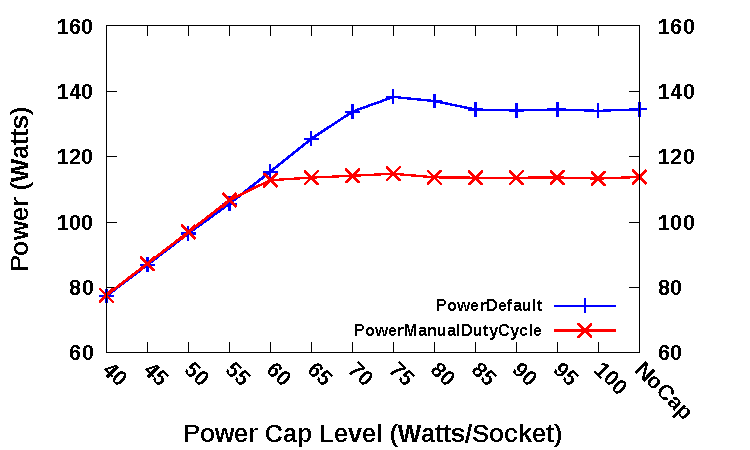
\includegraphics[width=3.5in]{fake-power.pdf}
%    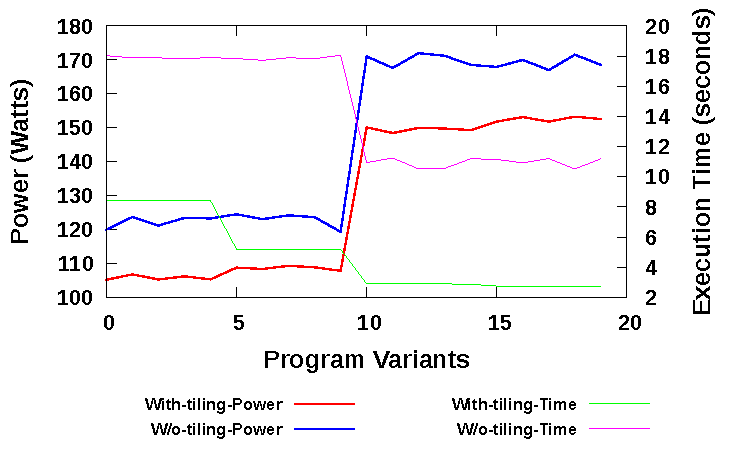
\includegraphics{Covariance}
    \caption{Power }
    \label{fig:Unbalanced-fake}
\end{figure}
\begin{figure}[bt]
    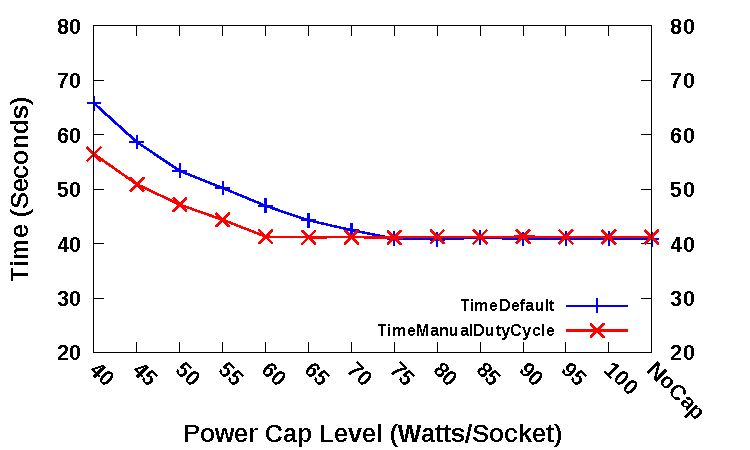
\includegraphics[width=3.5in]{fake-time.pdf}
%    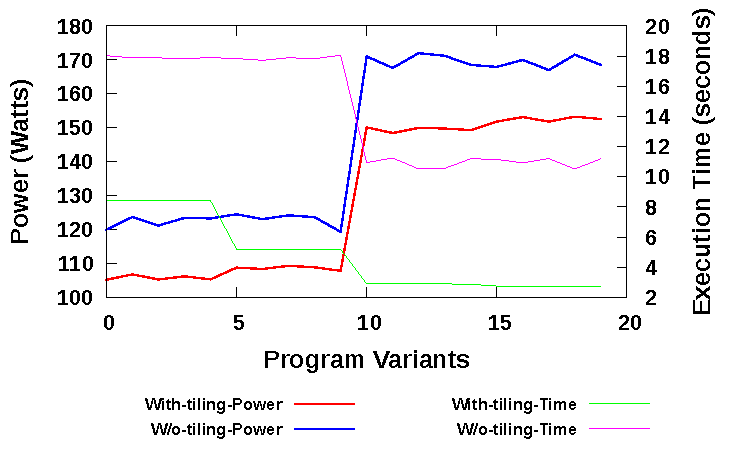
\includegraphics{Covariance}
    \caption{Time}
    \label{fig:UnbalancedTime-fake}
\end{figure}

In light of the difference, trying to set duty cycle in a destroyed world, actually could save some power.
But the power is still higher than the default (see the following graphs). 
It seems that for OpenMP this approach has no hope. 
Thus, community detection code cannot benefit from such technique, although MPI seems to have benefited a lot. 


\begin{figure}[bt]
    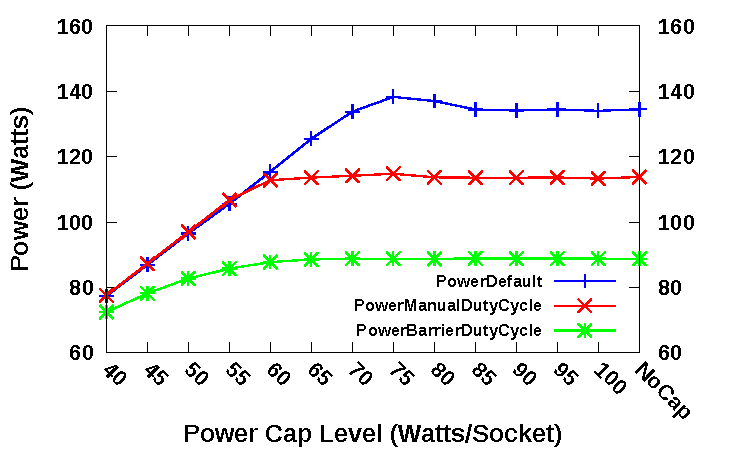
\includegraphics[width=3.5in]{fake2-power.pdf}
%    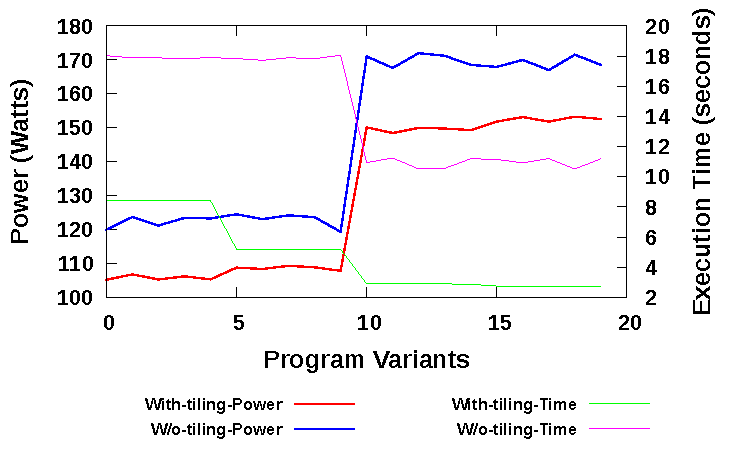
\includegraphics{Covariance}
    \caption{Power }
    \label{fig:Unbalanced-fake2}
\end{figure}
\begin{figure}[bt]
    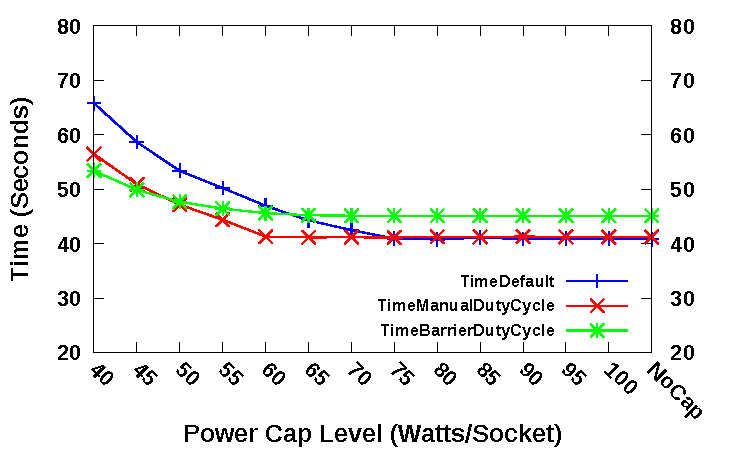
\includegraphics[width=3.5in]{fake2-time.pdf}
%    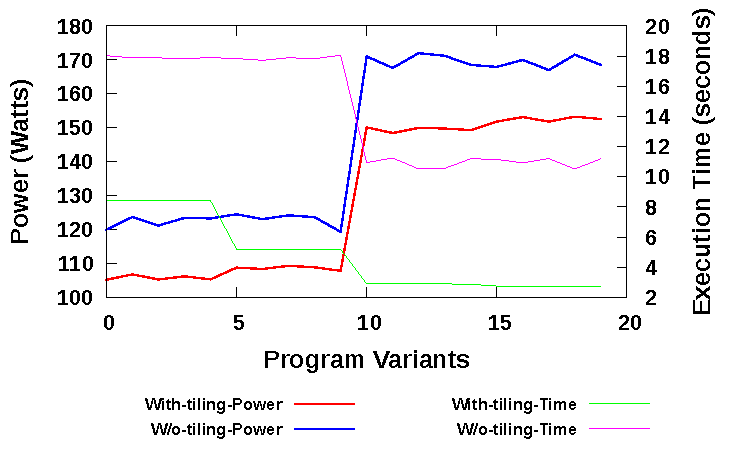
\includegraphics{Covariance}
    \caption{Time}
    \label{fig:UnbalancedTime-fake2}
\end{figure}


